\chapter{\label{results}Results}
\thispagestyle{fancy}

\section{Requirements Analysis}

The first step of the development process was to find out and define
how the solution should work. In collaboration with the Init7 network
engineering team, the core use cases were defined. As this was only
a proof of concept, the use cases were only described in a brief and
concise format. Furthermore, a consensus was formed how an engineer
should be able to operate with the plugin in general.

The following use cases were defined based on the design idea that
the engineer is able to write configuration templates which utilize data
available in NetBox, which subsequently can be deployed to a device.

\begin{enumerate}[label=U.\arabic*]
  \item{\label{uc-agg}} \textbf{Data Aggregation} 
  The engineer is able to easily configure and discover the available
  context information for authoring a template.
  \item{\label{uc-tmpl}} \textbf{Template Authoring}
  A view with an editor exists to author configuration templates.
  This view also provides a preview of the context data and this data
  can be used to preview the rendered template.
  \item{\label{uc-appl}} \textbf{Configuration Deployment}
  The engineer is able to apply a previously configured template
  to a network device.
  \item{\label{uc-cred}} \textbf{Credential Management}
  An authorized engineer is able to configure credentials which are used
  in the configuration deployment. The usage access to these credentials must
  be restrictable to specific users or groups. The ability to modify these
  credentials must also be restrictable to specific users or groups.
\end{enumerate}

In addition to the use cases, a decision has to be made on which
configuration method is used. In order to do this, the following compatibility
matrix was created:

\begin{center}
\begin{tabular}{l|c|c|c|c}
  Vendor & CLI & SNMP & NETCONF/YANG & HTTP API \\
  \hline\hline
  Cisco & Yes & Yes & Yes & No \\
  \hline
  MikroTik & Yes & No\textsuperscript{1} & No & Yes \\
  \hline
  Juniper & Yes & Yes & Yes & Yes \\
  \hline
  Extreme Networks & Yes & Yes & Yes & Yes \\
  \hline
  FS & Yes & No\textsuperscript{1} & Yes & Yes \\
  \hline
  Nokia & Yes & N/A & Yes & N/A \\
  \hline
  Ubiquity & Yes & No\textsuperscript{1} & No & Yes \\
\end{tabular}
\end{center}

\textsuperscript{1} SNMP is supported, but only supports read
operations, which makes it unsuitable for configuration deployment.

The above list of vendors include both vendors which are used within Init7
and other vendors which often appear in enterprise and ``power user''
environments. (Basic consumer hardware was disregarded since they usually
do not provide any standardized way to configure them.)

\paragraph{Configuration method decision} The HTTP APIs were excluded first
from the selection, since after some research, it became clear that they
differ wildly between vendors which makes it near impossible to write
a generic solution for. SNMP was excluded for both its age and lack
of write support in many vendor implementations. In the end, NETCONF/YANG was
chosen over the CLI because of the benefit of the model driven configuration
outlined in \ref{theory:conf:yang}.

\section{Application structure / Architecture}

To bridge the gap between the inventory management provided by NetBox and communicating with the actual hardware,
the solution is divided into layers.
In order to facilitate authentication and authorization there is the ``Credential Access Manager'' which communicates
with an external credential store. The access manager provides a user interface to enter and manage credentials, as well
as restricting who has access to these credentials by integrating into the NetBox permission system.
The ``Device Context Provider'' enables a user to define what information for a specific device shall be pulled.
Using the existing GraphQL API provided by NetBox, the user can easily identify what information is available and how it is
accessed. After the context data is defined it will subsequently be used in the ``Configuration Template Editor''
where the user writes a template using the previously defined context data. This template can then be applied to
a class of devices utilizing constraints such as tags or locations.
Lastly, the ``Configuration Transport'' module pulls the configuration template and the credentials for a specific device
and pushes it to the actual device.


\begin{figure}[h]
  \centering
  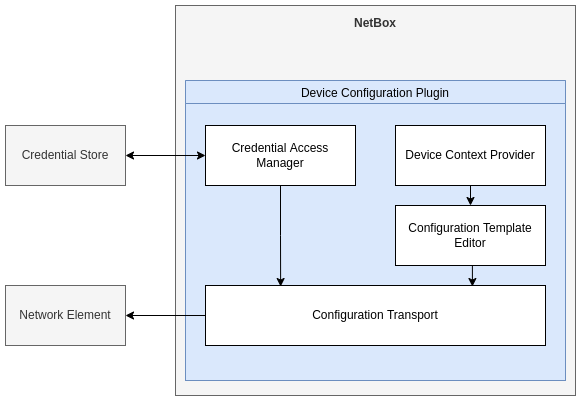
\includegraphics[width=0.8\textwidth]{Software-Arch}
  \caption{Software Architecture Concept}
  \label{fig:soft-arch}
\end{figure}



\subsection{Credential Access Manager}

In order to offload parts of the potential security issues with storing
credentials, an external credential manager is used.
In this case, HashiCorp Vault is used, as it is relatively easy to
set up and became one of the de facto solutions in multiservice
environments. To integrate Vault into the NetBox plugin, the client
library \icode{hvac} is used. A small abstraction layer is built
on top of the library, to make it easy for the rest of the plugin
to store and retrieve secrets.

\subsection{Device Context Provider}

Rendering templates in general usually requires some sort of context data
(i.e. a template for a marketing mail might require the customers name.)
NetBox already has a functionality called ``Export Templates'' which
allow a user to write templates to export lists of data with a custom
output format. What makes these ``Export Templates'' hard to use is that
they utilize the python objects mapped from the database as context,
which makes it somewhat necessary to know the internals of NetBox to
use them effectively.

Though what NetBox also provides, is a GraphQL API. GraphQL allows
the API consumer to specify exactly what data one is interested in,
in addition to requiring a complete specification for the API.
Using this specification, one can use a client like ``GraphiQL'',
which provides the user with autocompletion and documentation
access. As this client is built-in to NetBox, it provides an
intuitive user interface for specifying context data.

The Device Context Provider is therefore implemented by accepting
GraphQL queries in its configuration, which the user can author
with ``GraphiQL''.

\subsection{Configuration Template Editor}

Since the template the user writes should result in a valid NETCONF RPC
message, which is constructed using XML syntax, a code editor like experience
is preferred. Since NetBox is a browser based application, JavaScript based
code editors were evaluated and the Ace editor was chosen based on its
lightweightness and simplicity.

The template editor is split into three panes, where the engineer can see
the context data, the template content and a preview. This way, the engineer
is always aware what context data he can use, and can quickly see what the result
of a rendered template looks like.

\subsection{Configuration Transport}

Lastly, the configuration transport component ties all the other components
together and enables the deployment of a configuration to a device.
The actual deployment is implemented through the \icode{ncclient} library,
which manages the NETCONF connection and supplies an interface to send
RPCs through it.

Additionally, the ``glue'' is implemented to facilitate the rendering of
the template, retrieving the credentials and subsequently deploying the
configuration.
Special care needs to be taken when retrieving the credentials, as the
configured authorization needs to be enforced to prevent users from
deploying configuration when they are not allowed to do so.


\section{\label{eval-security}Security Evaluation}

To evaluate the security of the implemented solution, scenarios based on
the threat actors defined in \ref{method:eval-sec} were drawn up and
subsequently checked.


\begin{enumerate}[label=S.\arabic*]
  \item An {\it external actor} only with the knowledge
  that the system exists, cannot gain any form of access to the system or infrastructure. \\
  NetBox is behind a firewall which only allows access from within the company network.
  Additionally, NetBox is protected with standard username and password authentication,
  which has currently no known exploits for the latest version of Django (the web framework NetBox is based on).
  The impact is therefore negligible.

  \item An {\it external actor} gains non-elevated privileges to the server NetBox is running on. \\
  In a standard NetBox deployment, the instance is running as a separate user or even within a container.
  Low privilege access on Linux inspect memory of other processes, therefore the stored credentials
  cannot be extracted. If the actor has access to the configuration files, he may be able to discover the credentials of the
  database NetBox uses. In that case, the actor may be able to create a user within NetBox and gain administrative access
  to the running instance. While the actor is now able to deploy configurations to devices using the existing credentials,
  the credentials themselves cannot be extracted, as the secret, once stored, is never revealed to any user ever again.
  The privilege escalation within NetBox can be prevented through proper access restrictions to both the database
  and configuration data.
  The impact is high, but with proper configuration it can be significantly reduced.

  \item An {\it unauthorized employee} without any explicit privileges attempts to deploy a configuration to a device. \\
  The employee is not able to trigger a deployment because of the authorization check at the credential access manager.
  But, the employee is able to modify configuration templates, potentially tricking an authorized user to deploy it to a device.
  This is something that was missed during development and must be fixed before usage in production.

  \item An {\it unauthorized employee} with only usage access on specific credentials attempts to change the authentication information,
  potentially causing a denial of service for the operation of the configuration management. \\
  This is prevented through the authorization check in the credential access manager. The main risk is misconfiguration within the
  credential access manager if too permissive privileges are set.

\end{enumerate}

\section{Scenario Evaluation}

The following sections describe two chosen real-world scenarios within Init7.
More specifically, they are services which can be ordered by customers and also
require some manual work by network engineers in the current process.

The goal is to show how manual labor can be replaced or supported by the
created NetBox plugin.

\subsection{Fiber7}

Fiber7 is Init7's flag-ship product in the private consumer space,
providing consumers a \acrshort{P2P} fiber-optical connection directly into
Init7 infrastructure. Since this is the most commonly sold product by Init7
it is already one of the most streamlined processes throughout the department
with work being largely automated.

\begin{figure}[h]
  \centering
  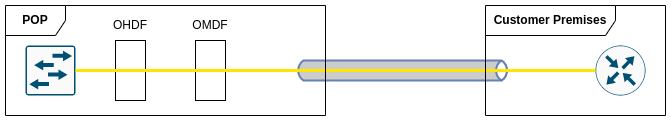
\includegraphics[width=\textwidth]{P-Fiber7}
  \caption{Fiber7 Service Diagram}
  \label{fig:fiber7}
\end{figure}

When the work-order arrives at the network engineer, it has already been decided
or defined at which \acrshort{POP}, network switch and interface the customer
will be connected to. The engineer will then go through the following process:

\begin{enumerate}
  \item A new service configuration ticket arrives
  \item Verify that there is no other active use on the chosen interface
  \item Apply the default configuration profile for Fiber7 private customers on the interface
  \item If the customer requested a static IP address, configure it on the DHCP server
  \item If the customer requested a prefix, configure it on the router connected to the switch
  \item If the customer does not specify a specific service activation date, enable the switchport
  \item Update NetBox with the performed configuration
  \item Update the service configuration ticket
\end{enumerate}

While the process might have seven steps, usually not all of that work is required.
When choosing the interface for the new service, it is verified through the \acrshort{OSS}
that the port has no other active use.
Interfaces have the Fiber7 private customer profile configured by default
if it was previously unused or was previously used for the same service,
rendering step 3 usually unnecessary.
Most commonly, customers do not request static IP addresses or prefixes as
they are an additional cost to the subscription and are only used by ``power-users'',
rendering steps 4 and 5 unnecessary.

The key observation that can be made, is that there are multiple manual steps
which can be prone to mistakes, yet they are always performed the same way. This makes
them good candidates for automation. Thus, the goal is to restructure the process
to the following:

\begin{enumerate}
  \item A new service configuration ticket arrives
  \item Within NetBox:
  \begin{enumerate}
    \item Set the service field on the interface to Fiber7
    \item 
  \end{enumerate}
\end{enumerate}

\cn{(above) list not complete}

\cn{Describe process to extract template information}

\cn{Describe verification}

\subsection{Business Optical Service}


\begin{figure}[h]
  \centering
  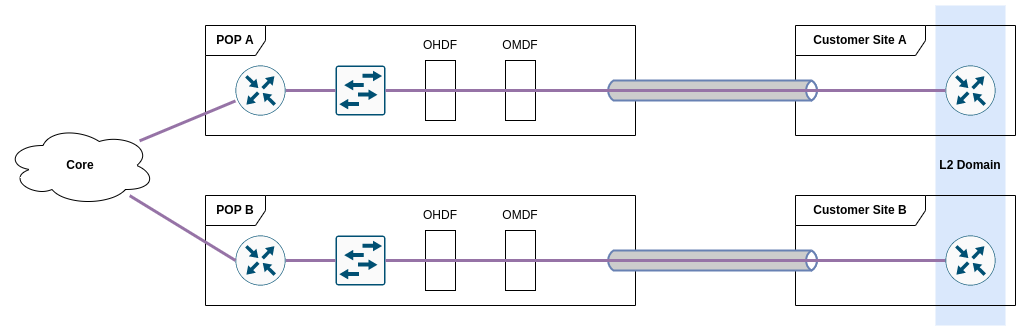
\includegraphics[width=\textwidth]{P-S2S}
  \caption{Business Optical Service Diagram}
  \label{fig:s2s}
\end{figure}

\cn{
 - B2B customer (standard)
  - Access Port with less configuration  \\
  - VLAN 600  \\
  - Static IP on router  \\
  - Static Route on router  \\
 - B2B customer (new)  \\
  - Trunk Port  \\
  - Allowed VLAN 600  \\
  - + same as standard?  \\
 - B2B Site-2-Site  \\
  - VLL through MPLS  \\

 - MikroTik ZTE  \\
 }